This element simulates a beam-driven monopole mode cavity using the fundamental theorem of beam loading and phasor rotation.
In addition, a generator-driven field may be included using a feedback system \cite{Berenc-IPAC15-MOPMA006}.

Note on phase conventions: the phase convention for the \verb|PHASE_SETPOINT|  parameter of \verb|RFMODE| is the
same as for the \verb|PHASE| parameter of \verb|RFCA|. However, in the output files from \verb|RFMODE|, i.e., the
files requested with the \verb|RECORD| and \verb|FEEDBACK_RECORD| parameters, a different convention is used, which 
differs by $-90$ degrees from the \verb|PHASE_SETPOINT|  parameter. 

The feedback implementation uses either amplitude and phase feedback or else in-phase and quadrature feedback.
It is active when a non-zero value is given for \verb|DRIVE_FREQUENCY| and when either
\verb|AMPLITUDE_FILTER| and \verb|PHASE_FILTER| or else
\verb|IN_PHASE_FILTER| and \verb|QUADRATURE_FILTER| are given.
Figure \ref{fig:rfFeedbackModel} shows the model used for the feedback system.
More information is available in \cite{Berenc-IPAC15-MOPMA006}.

\begin{figure}[htb]
\center
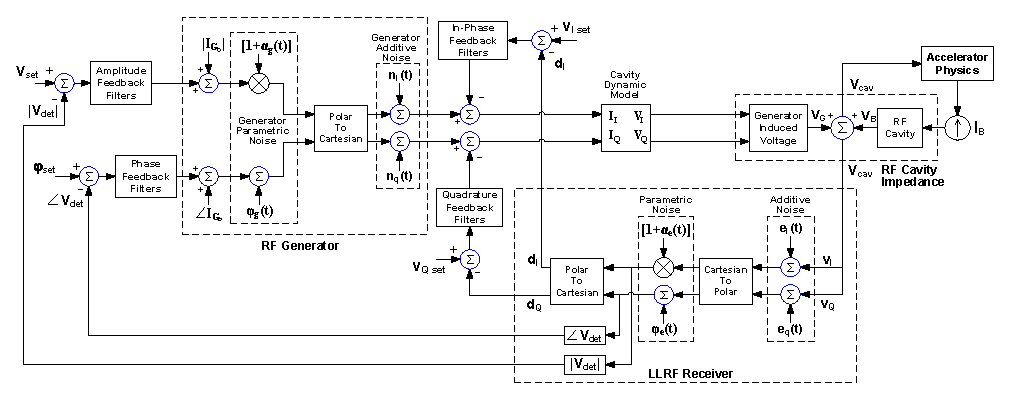
\includegraphics{rfFeedbackModel}
\caption{Rf feedback model used by the {\tt RFMODE} element.}
\label{fig:rfFeedbackModel}
\end{figure}

Normally, the field dumped in the cavity by one particle affects trailing particles in the same turn.
However, if one is also using a \verb|WAKE| or \verb|ZLONGIT| element to simulate the short-range wake of the cavity, this would be double-counting.
In that case, one can use \verb|LONG_RANGE_ONLY=1| to suppress the same-turn effects of the \verb|RFMODE| element.

Two output files are available: the \verb|RECORD| file includes bunch-by-bunch data on the beam-induced fields and the total cavity fields.
The \verb|FEEDBACK_RECORD| file includes tick-by-tick data from the feedback system simulation; {\em writing this file this can significantly impact performance.}

NB: when \verb|BUNCHED_BEAM_MODE| is set to a value other than 1, in order to obtain the effect of several bunches while tracking
only one bunch, the total charge set with the \verb|TOTAL| parameter of the \verb|CHARGE| element should equal the charge in
a single bunch, not the entire beam. However, when \verb|BUNCHED_BEAM_MODE|=1 (allowing an indeterminant number of bunches to be
actually present), then \verb|TOTAL| should be the total for all bunches together.
